\documentclass[xcolor=dvipsnames,aspectratio=169,12pt]{beamer}

\usepackage{tsbeamer}

\title{Democratic and Constitutional Regression under Populist Government}
\subtitle{An Empirical Analysis}
\author{Jasmin König and Tilko Swalve}
\date{\today}

\begin{document}

\maketitle


% special issue Leviathan, a theory outlet
% surprised we have graphs
% issue's theme is democratic regression


%%%%%
\frameprinciple{Democratic regression}{Democratic regression describes the decline of the quality of democracy.}
%%%%%

% tell the story of the book, democratic regression, related to the simultaneous increase in popularityof populist parties
%%%%%
\begin{frame}{Waves of democratic regression (Schäfer und Zürn, 2021)}
    \centering
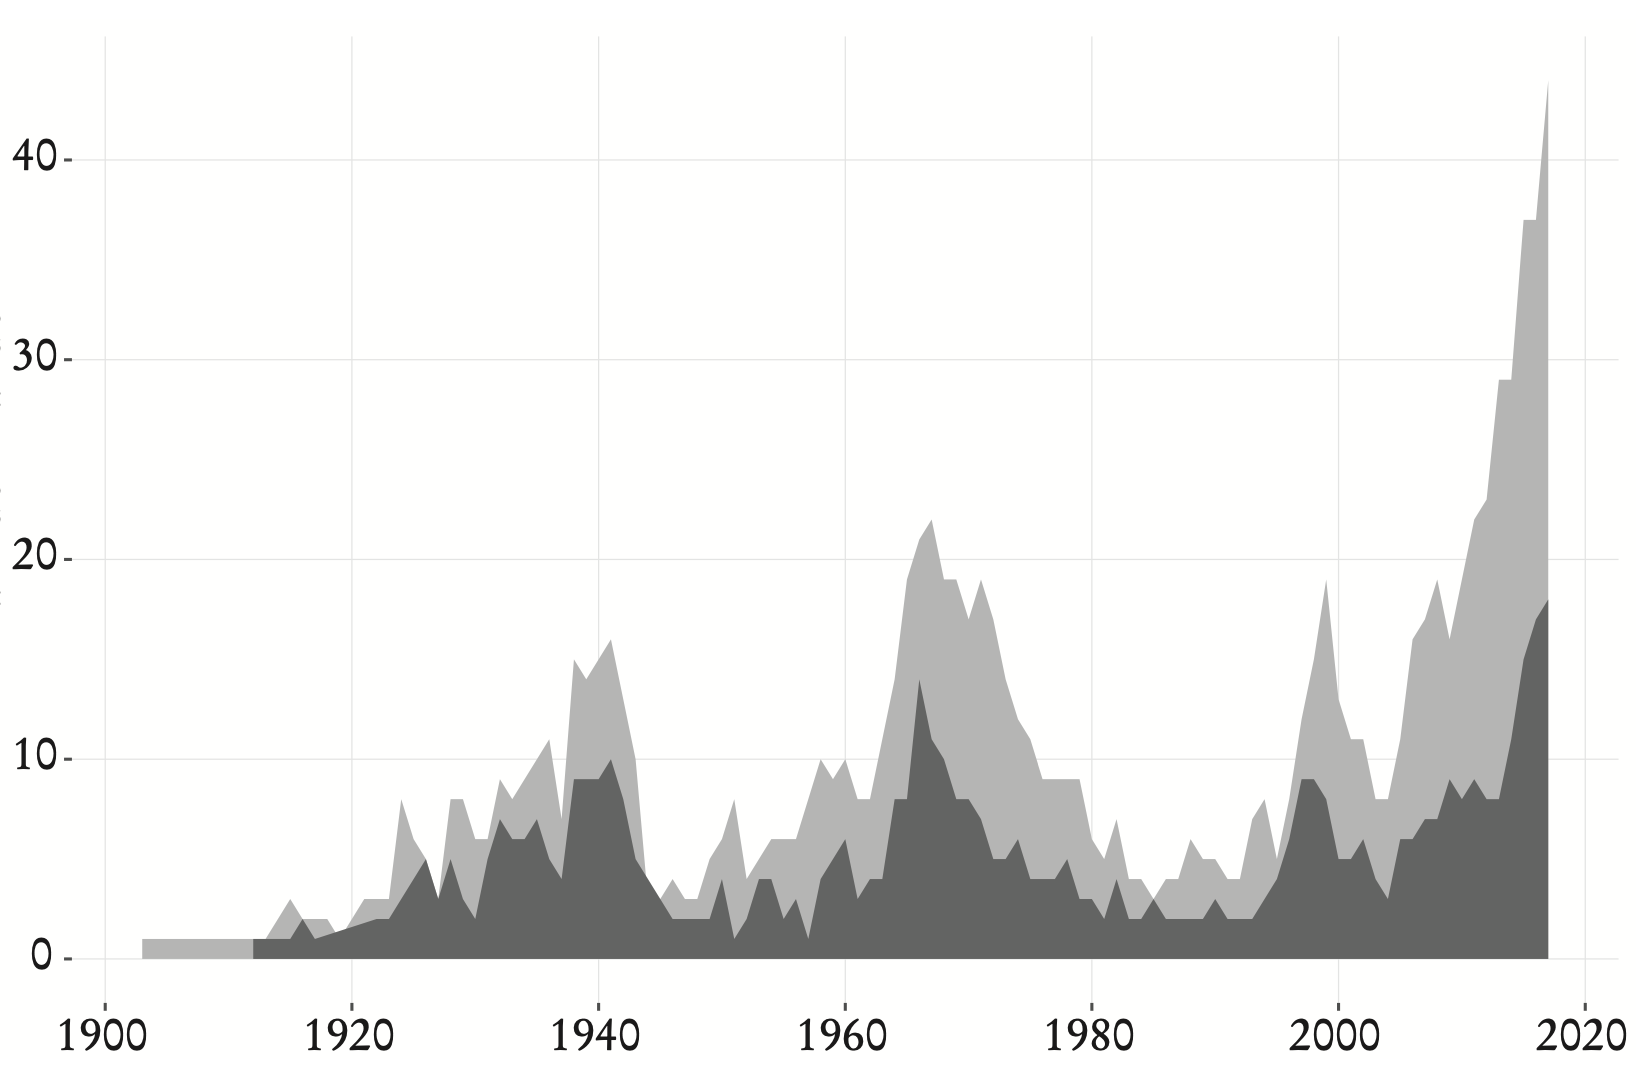
\includegraphics[width=0.8\textwidth]{fig/democraticregression}
\end{frame}
%%%%%

% in this context, examples like poland or hungary that we will look at a later stage of the talk are presented as evidence for the general trend
%%%%%
\frametitleslide{fig/polandII.png}{

}
%%%%%


% but there are some caveats, 
%%%%%
\begin{frame}{Measuring democratic regression is challenging}
    \textbf{Objective measures}
\begin{itemize}
    \item formal democratic institutions, such as presence of elections, a formal separation of powers, etc.
    \item minimal definition of democracy
    \item but: formal institutions vs democratic practice
\end{itemize}
\textbf{Subjective measures}
\begin{itemize}
    \item surveys (e.g. V-Dem): How well are the principles of liberal democracy implemented in your country?
    \item broader definition of democracy
    \item but: quality of democracy essentially determined by a survey among political science professors
    \item anchoring, differential item functioning etc.
\end{itemize}  
\end{frame}
%%%%%

%%%%%
\frameprinciple{Constitutional regression}{

Constitutional amendments that lead to a decline of the quality of democracy

}
%%%%%


%%%%%
\begin{frame}{}
\begin{wideitemize}
    \item What is the relationship between democratic regression and constitutional amendments?
    \item Do constitutional amendments by populist governments lead to a decline in the quality of democracy?
    \item Goal: Give subjective measures of democratic quality (V-Dem) a foundation of observable, objective events (constitutional amendments)
\end{wideitemize} 
\end{frame}
%%%%%

%%%%%
\begin{frame}{Populism and constitutional regression}

    \begin{wideitemize}
        \item Populism as a \textit{thin} ideology
        \begin{itemize}
        \item the will of the people (majority)
        \item people are homogenous
        \item the elites prevent the will of the people to prevail
        \end{itemize}
        \item clashes with key tenets of liberal democracy
        \begin{itemize}
            \item countermajoritarian institutions
            \item protection of minority rights
        \end{itemize} 
    \item populism often described as a threat to liberal democracy
    \item but: some authors stress positive effects of populism, such as increasing participation of underpriviledged social groups 
\end{wideitemize}
\end{frame}
%%%%%


%%%%%
\begin{frame}{Data}
    \begin{wideitemize}
        \item 40 European and  19 Latin American countries between 1991 and 2021, excluding autocracies
        \item \textbf{Dependent variables}
        \begin{itemize}
        \item index of liberal democracy (V-Dem,continuous, 0-1)
        \item index of civil society participation (V-Dem, continuous, 0-1)
        \end{itemize}
        \item \textbf{Independent variables}
        \begin{itemize}
            \item constitutional event (Comparative Constitutions Project, binary)
            \item weighted populism score of government (V-Party, constructed by us, continuous, 0-1)
            \item geographical indicator (Latin America), year fixed effects
        \end{itemize}
    \end{wideitemize} 
\end{frame}
%%%%%

%%%%%
\begin{frame}{Descriptive Statistics I}
\begin{wideitemize}
    \item 1740 country-year observations
    \item Constitutional changes are \textit{relatively} rare: 595 observations with changes, 1088 without
    \item Constitutional changes by populist governments are even more rare: 75 observations of constitutional changes by governments with a populism score of $>0.5$
\end{wideitemize} 
\end{frame}
%%%%%

%%%%%
\begin{frame}{Descriptive Statistics II}
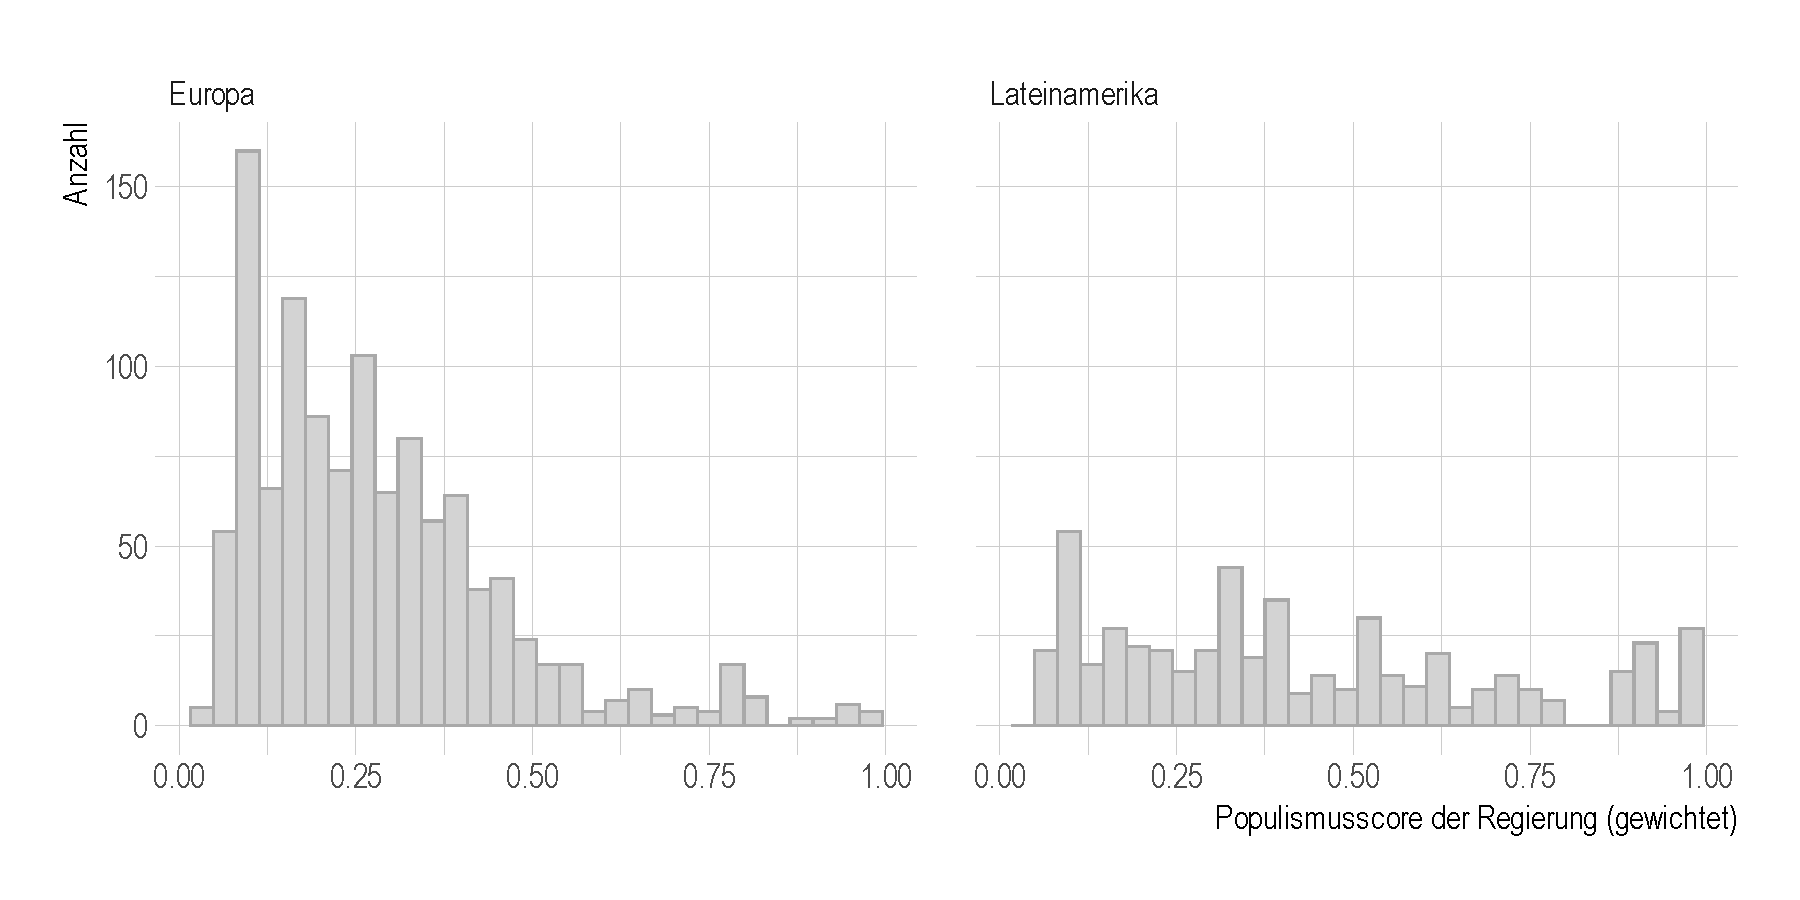
\includegraphics[width=1\textwidth]{fig/populismscorehist}
\end{frame}
%%%%%

%%%%%
\begin{frame}{Estimation}
\begin{wideitemize}
    \item OLS regression with year fixed effects
    \item Model 1 (Europe only): interaction effect between constitutional amendment and populism score
    \item Model 2: tripel interaction between constitutional amendment, populism score and Latin America dummy
\end{wideitemize} 
\end{frame}
%%%%%

%%%%%
\begin{frame}{Results (Model 1)}
    \centering
    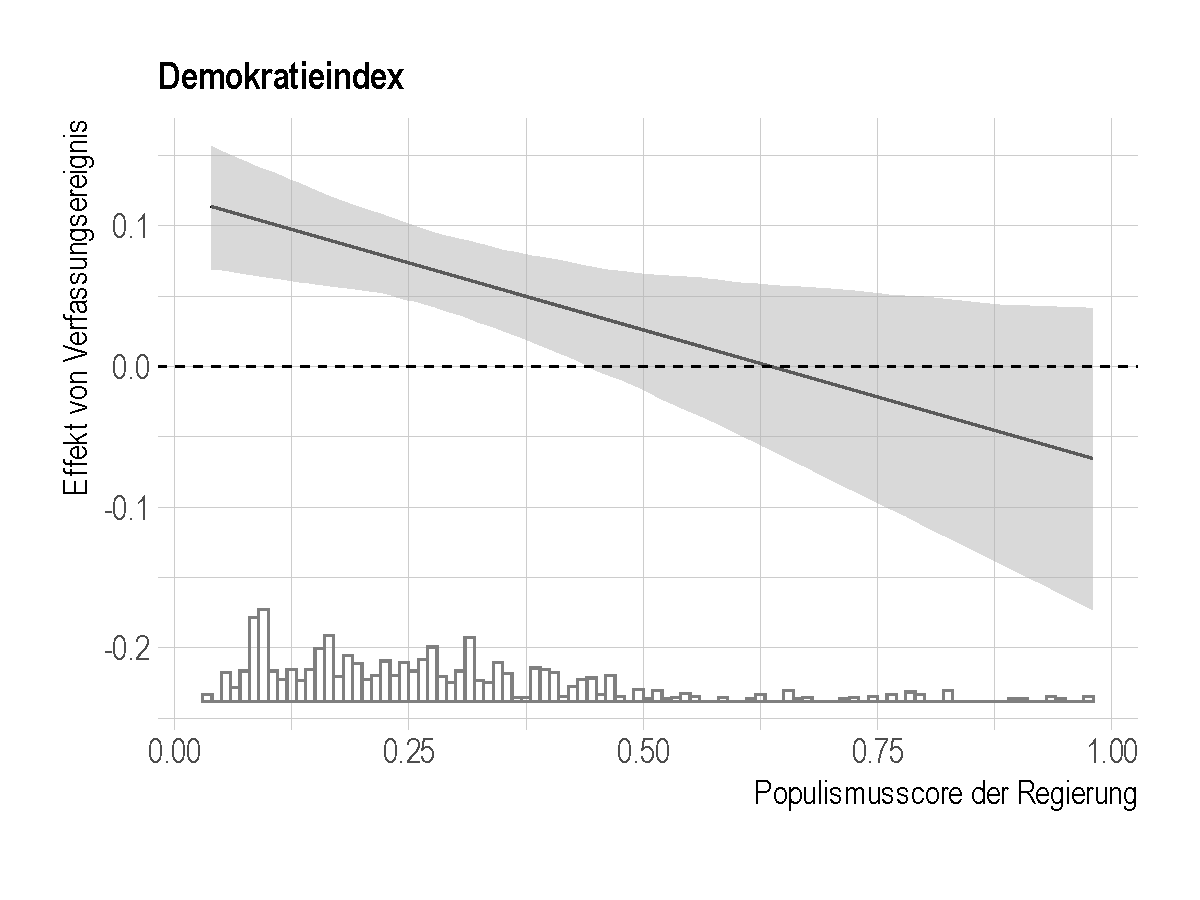
\includegraphics[width=0.8\textwidth]{fig/populismscoreregI}
\end{frame}
%%%%%

%%%%%
\begin{frame}{Results (Model 1)}
    \centering
    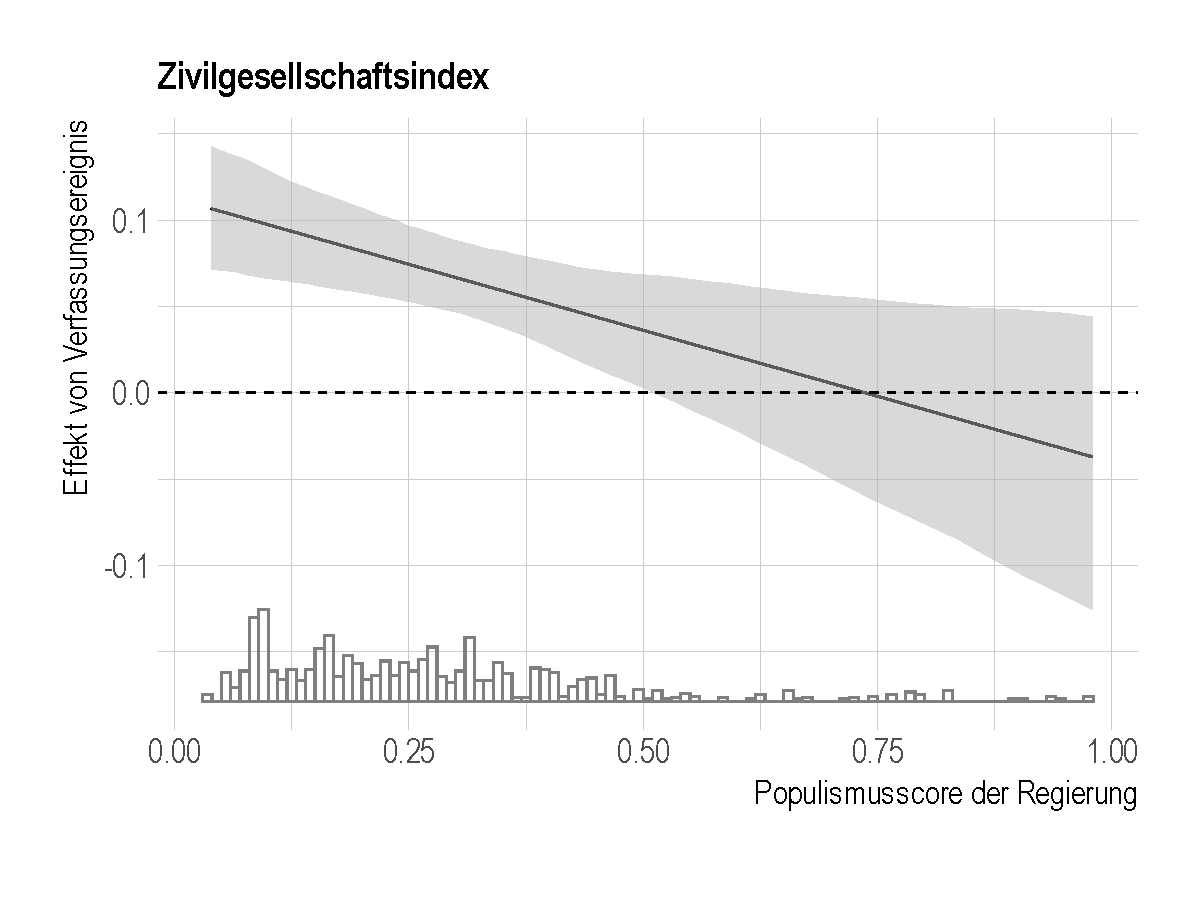
\includegraphics[width=0.8\textwidth]{fig/populismscoreregII}
\end{frame}
%%%%%

%%%%%
\begin{frame}{Results (Model 2)}
    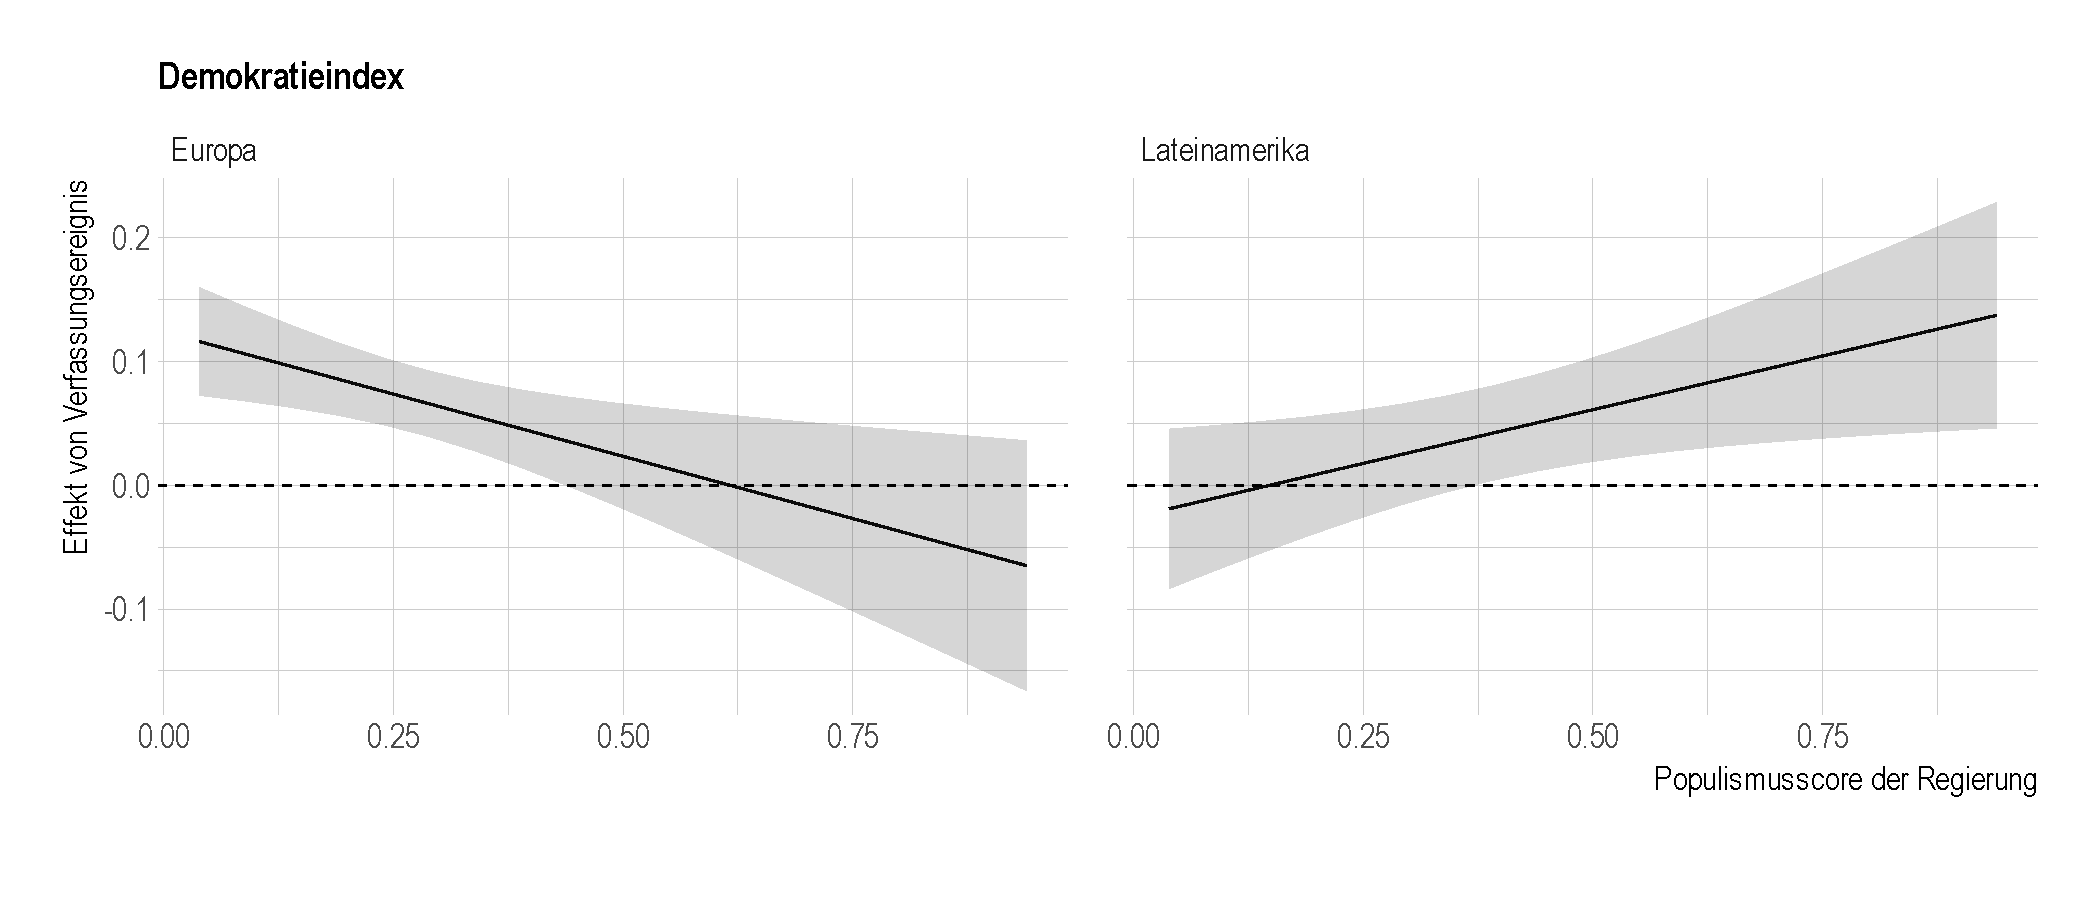
\includegraphics[width=1\textwidth]{fig/populismscoreregIII}
\end{frame}
%%%%%


%%%%%
\begin{frame}{Results (Model 2)}
    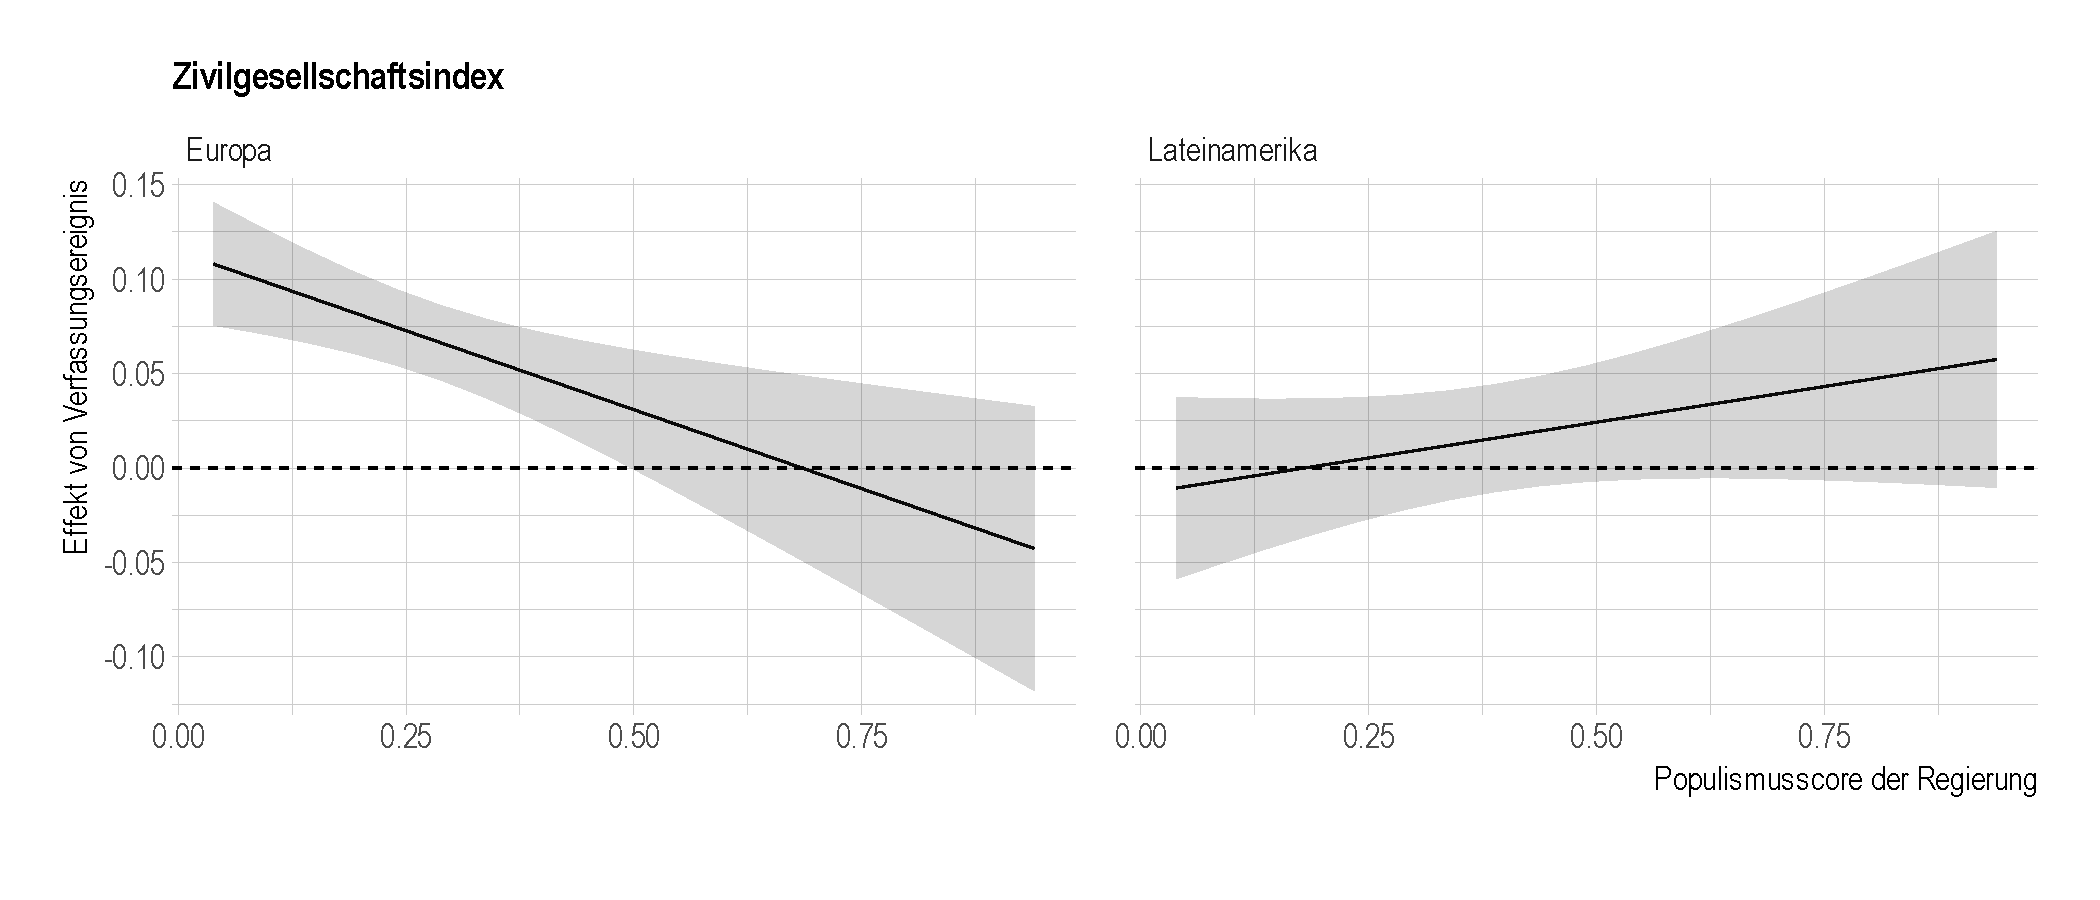
\includegraphics[width=1\textwidth]{fig/populismscoreregIV}
\end{frame}
%%%%%

%%%%%
\begin{frame}{Further results}
    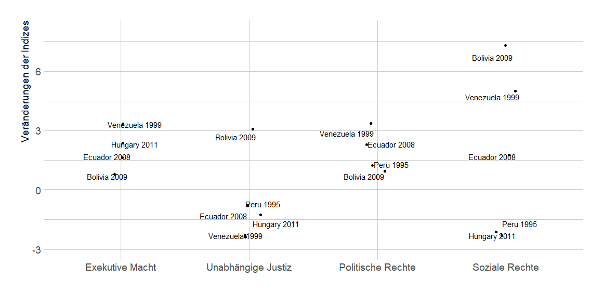
\includegraphics[width=1\textwidth]{fig/moreresults}
\end{frame}
%%%%%

%%%%%
\begin{frame}{Conclusions large-N analysis}
\textbf{Model I}    
\begin{wideitemize}
    \item negative interaction between constitutional amendment and populism score
    \item but: no negative effect on liberal democracy index or civil society index
\end{wideitemize} 
\textbf{Model II}
\begin{wideitemize}
    \item heterogeneous effects across regions
    \item populist constitutional amendments can even have a positive effect on liberal democracy in Latin America
\end{wideitemize} 
\textbf{More results}
\begin{wideitemize}
    \item where populist amendments had a negative impact, it focused on enlarging executive powers, decreasing judicial independence
\end{wideitemize} 
\end{frame}
%%%%%

%%%%%
\frameimportantpoint{

Democratic regression with and without constiutional regression: a case study

}
%%%%%

%%%%%%
\frameimageleft[0.4]{fig/hungaryI}{Hungary under Fidesz}{

    \begin{wideitemize}
        \item Orban's Fidesz party gained an absolute majority of votes and a 2/3-majority of seats in 2010
        \item fundamental changes to the institutional structure of the country since then
        \item illiberal democracy
    \end{wideitemize} 

}
%%%%%%

%%%%%%
\frameimageright[0.5]{fig/polandconst}{Poland under PiS}{

\begin{wideitemize}
    \item PiS wins the elections in 2015
    \item party prefers the Hungary-model: Budapest in Warsaw
    \item restructuring of the country's institutional setup 
\end{wideitemize} 

}
%%%%%%

%%%%%
\begin{frame}{Populism scores in Hungary and Poland}
    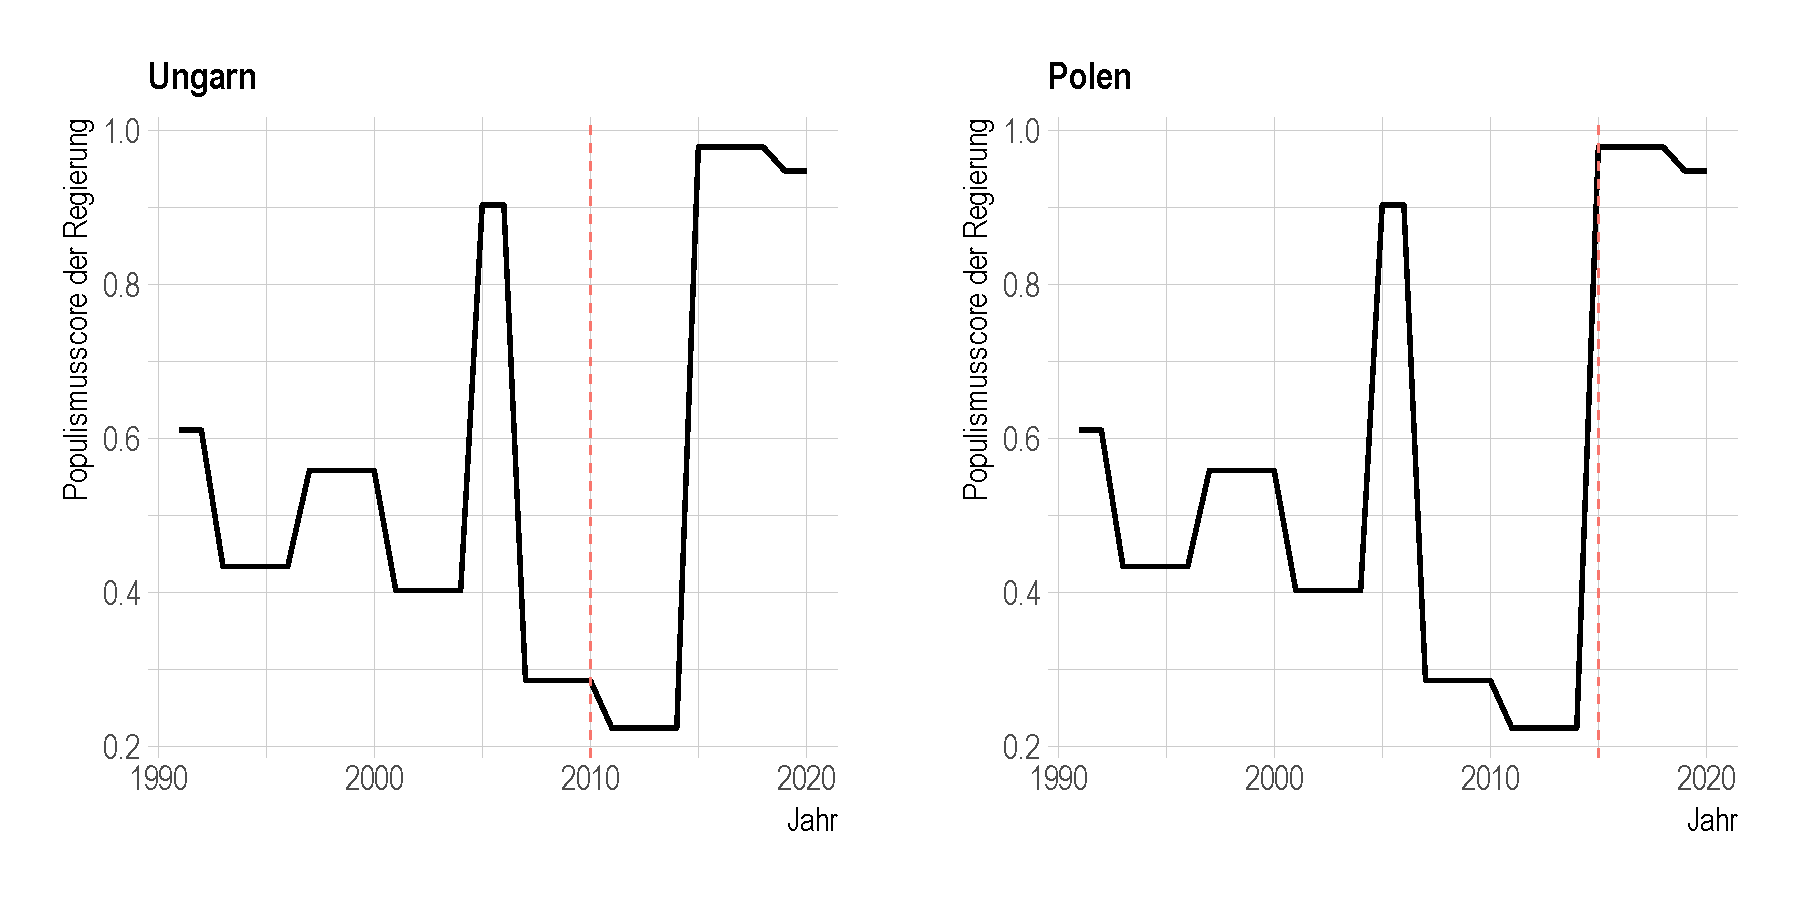
\includegraphics[width=1\textwidth]{fig/populboth}
\end{frame}
%%%%%

%%%%%
\begin{frame}{Liberal  democracy and constitutional events in Hungary and Poland}
    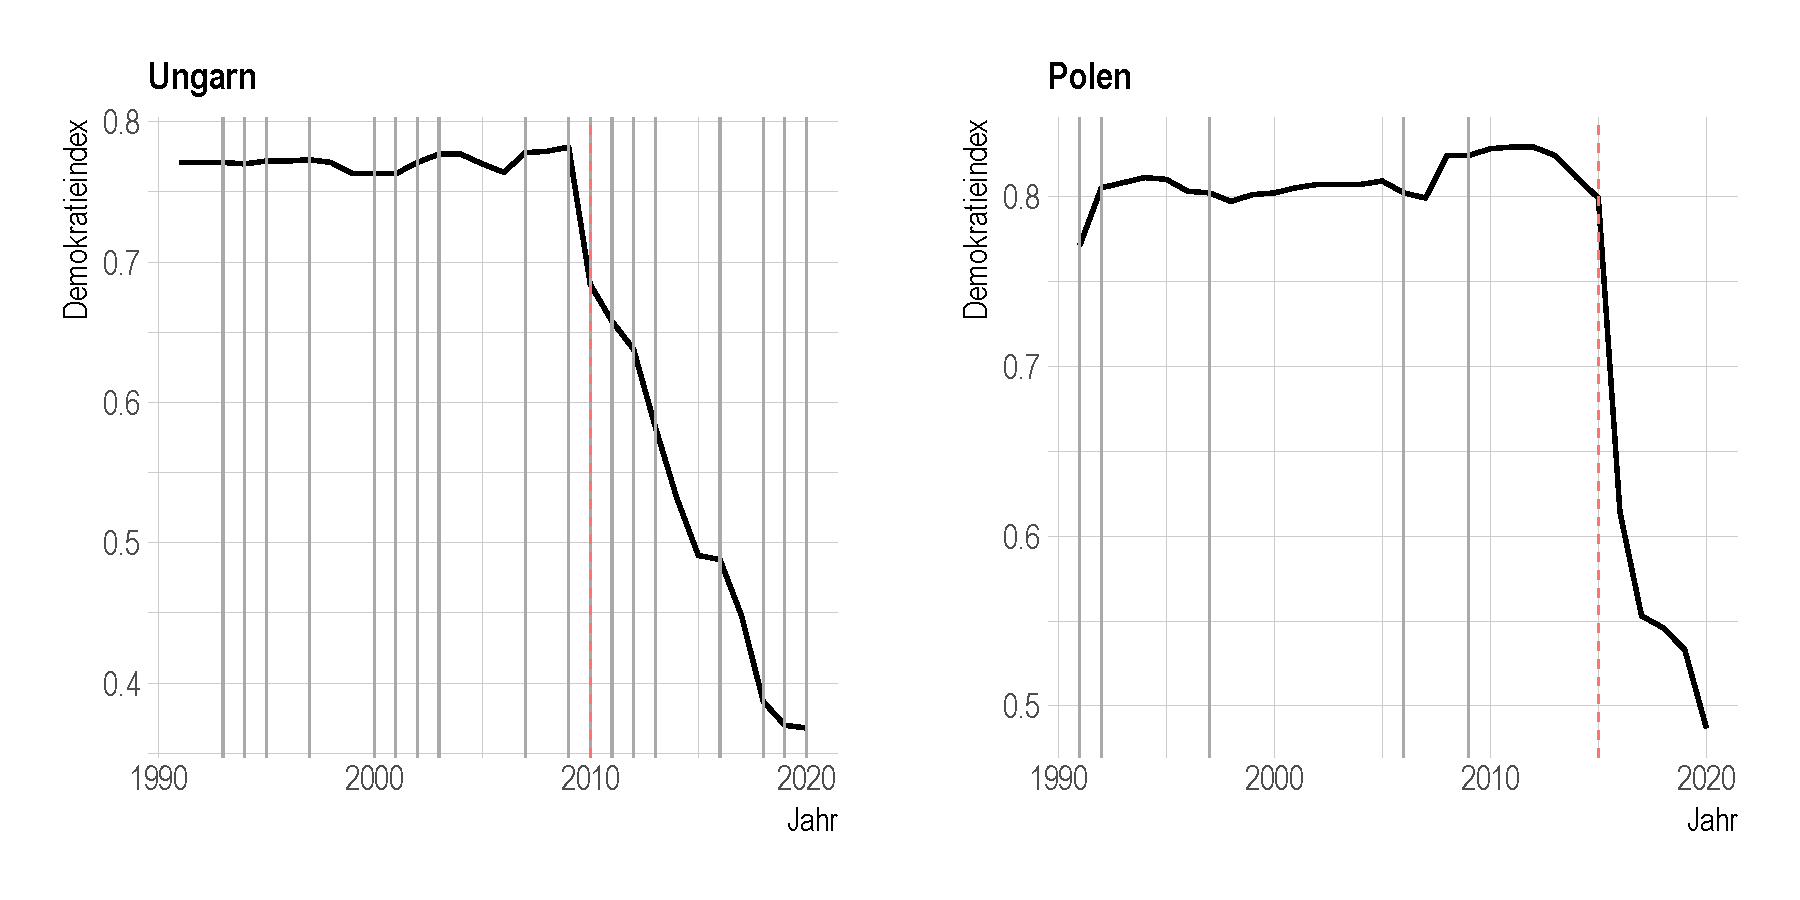
\includegraphics[width=1\textwidth]{fig/libdemboth}
\end{frame}
%%%%%

%%%%%
\begin{frame}{Conclusions case study}
\begin{wideitemize}
    \item formal constitutional regression is not a necessary condition for democratic regression
    \item the lack of electoral majorities to change the constitution can be overcome by packing the court, disabling its function, then pass laws that would breach the constitution under normal circumstances
    \item a naive focus on constitutional events only is insufficient
\end{wideitemize} 
\end{frame}
%%%%%

\end{document}